\documentclass{beamer} %use [handout] to get summary
\usepackage{pgfpages}
%\setbeameroption{show notes on second screen=left} %enable for notes
\usepackage{graphicx}
\usepackage{xcolor}
\usepackage{listings}
\usepackage{hyperref}
\lstset{language=python,frame=single}
\usepackage{verbatim}
\usepackage{subcaption}
\usepackage{amsmath}
\usepackage{relsize}
\usepackage{appendixnumberbeamer}
\usepackage{xparse}
\usepackage{multimedia}
\usepackage{tikz}
\usetikzlibrary{matrix,backgrounds}
\pgfdeclarelayer{myback}
\pgfsetlayers{myback,background,main}

\tikzset{mycolor/.style = {line width=1bp,color=#1}}%
\tikzset{myfillcolor/.style = {draw,fill=#1}}%
\tikzstyle{line} = [draw, line width=1pt]
\tikzstyle{arrow} = [draw, line width=1pt, ->]

\NewDocumentCommand{\highlight}{O{blue!40} m m}{%
\draw[mycolor=#1,rounded corners] (#2.north west)rectangle (#3.south east);
}

\NewDocumentCommand{\fhighlight}{O{blue!40} m m}{%
\draw[myfillcolor=#1,rounded corners] (#2.north west)rectangle (#3.south east);
}

\usetheme[numbering=fraction, background=dark]{metropolis}
%%\AtBeginSection[]
%%{
%%  \begin{frame}
%%    \frametitle{Table of Contents}
%%    \tableofcontents[currentsection]
%%  \end{frame}
%%}

%%\let\olditem\item
%%\renewcommand{\item}{\vspace{0.5\baselineskip}\olditem}

\newcommand{\E}[1]{\mathbb{E}\left[#1\right]}
\begin{document}

\title{Reinforcement Learning 2}
\subtitle{Complications \& approximations}
\author{Andrew Lampinen}
\date{Psych 209, Winter 2018}
\frame{\titlepage}


\section{Introduction}
\begin{frame}{Plan for this lecture}
Talk about all the stuff that makes it messy: 
\begin{center}
    \includegraphics[width=0.3\textwidth]{figures/walkingbaby.jpg}~
    \includegraphics[width=0.3\textwidth]{figures/selfdrivingcar.jpg}~
    \includegraphics[width=0.3\textwidth]{figures/playingchess.jpg}
\end{center}
\vspace{-1em}
\begin{itemize}
    \item<2-> Infinite spaces, approximation \& generalization.
    \item<3-> Correlations \& replay.
    \item<4-> Exploration \& on/off-policy learning.
    \item<5-> Hierarchies \& plans.
    \item<6-> Unobservables \& POMDPs, different assumptions and other approaches.
\end{itemize}
\end{frame}

\section{Function approximation}

\begin{frame}{Similarities \& dissimilarities}
\begin{itemize}
    \item Wheels of car can be at infinitely many angles, but is 0.55 radians really that different from 0.56?
    \item<2-> More state, action pairs in chess than atoms in observable universe. However: \vspace{0.5em} 
    \begin{center}
        \includegraphics[width=0.25\textwidth]{figures/simchess4.png}~
        \includegraphics[width=0.25\textwidth]{figures/simchess3.png} \\[5pt]
        \includegraphics[width=0.25\textwidth]{figures/simchess2.png}~
        \includegraphics[width=0.25\textwidth]{figures/simchess1.png}
    \end{center}
\end{itemize}
\note{Look at the similarity between these positions -- we should be able to generalize across them somehow (being aware that we shouldn't overgeneralize to the last case)}
\end{frame}

\begin{frame}{Approximating the Q-table}
\begin{itemize}
    \item Previously, the Q-table was a lookup function. Let's replace this with some other function that maps states and actions to Q-values.
    \begin{figure}
    \centering
    \begin{tikzpicture}
    \node at (0, 1) (B) {\includegraphics[width=0.12\textwidth]{figures/simchess2.png}};
    \node[draw, circle, minimum width=3em, line width=1pt] at (0, -1) (M) {Rd8};
    \node[draw, circle, minimum width=3em, line width=1pt] at (6, 0) (Q) {+0.743}; 

    \only<1|handout:0> {

        \node[draw, minimum width=3em, line width=1pt, text width=4em, align=center] at (3, 0) (LT) {Lookup table};
        \path [line] ([xshift=-4pt]B.east) to (LT.west);
        \path [line] (M.east) to (LT.west);
        \path [line] (LT.east) to (Q.west);

    }
    \uncover<2-> {
        \node[draw, circle, minimum width=3em, line width=1pt] at (3, -1.5) (H0) {};
        \node[draw, circle, minimum width=3em, line width=1pt] at (3, 0) (H1) {};
        \node[draw, circle, minimum width=3em, line width=1pt] at (3, 1.5) (H2) {};

        \path [line] ([xshift=-4pt]B.east) to (H0.west);
        \path [line] ([xshift=-4pt]B.east) to (H1.west);
        \path [line] ([xshift=-4pt]B.east) to (H2.west);
        \path [line] (M.east) to (H0.west);
        \path [line] (M.east) to (H1.west);
        \path [line] (M.east) to (H2.west);

        \path[line] (H0.east) to (Q.west);
        \path[line] (H1.east) to (Q.west);
        \path[line] (H2.east) to (Q.west);
    }
    \end{tikzpicture}
    \end{figure}
    \item<3-> Loss: \[L = \left(r_{t+1} + \gamma \max_{a'} Q(s_{t+1}, a'; \theta_i^{-}) - Q(s_{t}, a_t; \theta_i)\right)^2\]
\end{itemize}
\note{NNs are universal function approximators}
\end{frame}

\begin{frame}{Playing atari games}
\begin{center}
    \includegraphics[width=\textwidth]{figures/DQN.png}
\end{center}
\note{Note that the action is no longer an input! Why might this be better in practice?}
\end{frame}

\section{Replay}
\begin{frame}{Fix one problem and ...}
\begin{itemize}
    \item Generalization comes at the expense of cross talk and catastrophic forgetting. Will a self-driving car learning to parallel park forget how to drive on the freeway?
    \item<2-> CLS is a theory of how humans and animals avoid this:
    \begin{center}
        \includegraphics[width=0.75\textwidth]{figures/cls.jpg}
    \end{center}
\end{itemize}
\end{frame}

\begin{frame}{Replay buffers}
The Atari game-playing paper addressed this with \textbf{experience replay}:
\begin{itemize}
    \item Whenever we experience a new \((s_t, a_t, r_{t+1}, s_{t+1})\) tuple, stick it in a buffer.
    \item<2-> instead of  
         {
          \[\Delta Q^{\pi}(s_{t}, a_t) = \alpha \underbrace{\left( \left[ r_{t+1} + \max_{a'} \gamma Q^{\pi}(s_{t+1}, a') \right] - Q(s_t, a_t)\right)}_{\text{prediction error!}}\]}%
    \item<3-> we sample a random experience from our buffer and update with that: \(k \sim Unif(\text{replay buffer indices})\) 
         {
          \[\Delta Q^{\pi}(s_{k}, a_k) = \alpha \underbrace{\left( \left[ r_{k+1} + \max_{a'} \gamma Q^{\pi}(s_{k+1}, a') \right] - Q(s_k, a_k)\right)}_{\text{prediction error!}}\]}


\end{itemize}
\end{frame}

\section{Exploration and exploitation and on/off policy}
\begin{frame}{The need to explore}
\begin{center}
    \includegraphics[width=0.75\textwidth]{figures/googlemaps.png}
\end{center}
\begin{itemize}
    \item<2-> How do I trade off between \textbf{exploiting} the best path to lunch I've found so far and \textbf{exploring} my other options?
    \item<3-> In other words, how do we incorporate exploration into our policy?
    \item<4-> This is important -- remember convergence guarantees required \emph{every} state, action pair to be visited ``frequently.''
\end{itemize}
\end{frame}

\begin{frame}{The exploration-exploitation trade-off}
There is a \emph{fundamental} trade-off between exploring and exploiting:
\begin{itemize}
    \item<2-> Exploring wastes time trying things I'm pretty sure aren't good.
    \item<3-> Exploiting risks missing a great opportunity.
    \item<4-> We have to find some balance between these that results in good payoffs but still makes sure we don't miss too much.
\end{itemize}
\end{frame}

\begin{frame}{\(\epsilon\)-greedy}
\begin{itemize}
    \item One simple technique is just to choose actions randomly some small fraction \(\epsilon\) of the time. 
    \item<2-> The rest of the time, take the maximum \(Q\) action. 
    \item<3-> We call this \(\epsilon\)-greedy.
    \item<4-> We can also do clever things like \emph{anneal} \(\epsilon\) over training.
        \begin{itemize} 
        \item Act mostly randomly and explore a lot early in training.
        \item Act mostly greedily and exploit a lot late in training/in testing.
        \end{itemize}
    \item<5-> (There are other possibilities, e.g. using a softmax over Q values.)
\end{itemize}
\end{frame}

\begin{frame}{Exploit during testing or keep exploring?}
The point about testing vs. training is a little tricky... 
\begin{columns}
\column{0.5\textwidth}
\begin{itemize}
    \item<1-> Do chess players stop learning when they're playing for the world championship? 
    \item<2-> A self-driving car can't just be trained and set free -- destinations, roads, and laws are all evolving.
    \item<3-> What if my direct path to lunch was blocked by a building that was torn down? 
\end{itemize}
\column{0.5\textwidth}
    \begin{center}
    \only<1|handout:0>{
        \includegraphics[width = \textwidth]{figures/chess.jpg}
    }
    \only<2|handout:0>{
        \includegraphics[width = \textwidth]{figures/citystreet.jpg}
    }
    \only<3>{
        \includegraphics[width = \textwidth]{figures/googlemaps.png}
    }
    \end{center}
\end{columns}
\end{frame}

\begin{frame}{Non-optimality of \(Q\)-learning under exploration}
\begin{itemize}
    \item But \(Q\)-learning fundamentally assumes that we will be behaving completely greedily during training! Why?
    \item<2-> It's built into our computation of the Q-update: 
        \[\Delta Q^{\pi}(s_{t}, a_t) = \alpha {\left( \left[ r_{t+1} + \, {\color{red} \max_{a'}} \, \gamma Q^{\pi}(s_{t+1}, {\color{red}a'}) \right] - Q(s_t, a_t)\right)}\]
    \item<3-> If we want to behave optimally with a policy \(\pi\) that explores, we have to incorporate this policy into the learning rule:
        {\footnotesize \[\Delta Q^{\pi}(s_{t}, a_t) \; {\color{red} \stackrel{?}{=}} \; \alpha \left( \left[ r_{t+1} + \, {\color{red} \sum_{a'} p(a' | s_t, a_t, s_{t+1}, \pi)} \, \gamma Q^{\pi}(s_{t+1}, {\color{red} a'}) \right] - Q(s_t, a_t)\right)\]}
\end{itemize}
\end{frame}


\begin{frame}{SARSA}
\begin{itemize}
    \item One algorithm for doing this is SARSA. It works almost exactly like Q learning, except we store \((s_t, a_t, r_{t+1}, s_{t+1}, a_{t+1})\)
    \item<2-> and change our update from 
        \[\Delta Q^{\pi}(s_{t}, a_t) = \alpha {\left( \left[ r_{t+1} + \, {\color{red} \max_{a'}} \, \gamma Q^{\pi}(s_{t+1}, a') \right] - Q(s_t, a_t)\right)}\]
        to
        \[\Delta Q^{\pi}(s_{t}, a_t) = \alpha {\left( \left[ r_{t+1} + \gamma Q^{\pi}(s_{t+1}, {\color{red} a_{t+1}}) \right] - Q(s_t, a_t)\right)}\]
    \item<3-> Since our actions in the state are distributed according to \(\pi\), in expectation our \(Q\)-value updates will be as well.
\end{itemize}
\note{Note that many algorithms that are not \(Q\)-learning per se use \(Q\)-values...}
\end{frame}

\begin{frame}{On/off-policy}
This highlights an important, but somewhat orthogonal distinction: \vspace{-1.5em} 
\begin{itemize}
    \item<2-> Do we want to learn \textbf{on-policy}, that is, using the same policy we will be using during evaluation (like SARSA)?
    \item<3-> Or do we want to learn \textbf{off-policy}, that is, using a different policy during training than during evaluation (like \(Q\)-learning)?
\end{itemize}
\uncover<4->{There are tradeoffs!} 
\begin{itemize}
    \item<5-> \textbf{On-policy:} Can be faster, can be more stable. 
    \item<6-> \textbf{Off-policy:} Can learn from anything, even totally random play. This makes incorporating replay or changing \(\epsilon\) for more early exploration easier.
\end{itemize}
\end{frame}

\section{Hierarchies \& plans}
\begin{frame}{Plans = hierarchies of actions}
\begin{figure}
\centering
\begin{tikzpicture}
\node[draw, line width=1pt] at (0, 0) (A) {Excercise to stay healthy};
\only<2->{
    \node[draw, minimum width=3em, line width=1pt] at (0, -1) (B) {Run the dish today};
    \path [arrow] (A.south) to (B.north);
}

\only<3->{
    \node[draw, minimum width=3em,text width = 2.5cm, line width=1pt] at (0, -2.5) (C) {Put on running clothes};
    \path [arrow] (B.south) to (C.north);
}
\only<4->{
    \node[draw, minimum width=3em,text width = 2.5cm, line width=1pt] at (3, -2.5) (D) {Leave the house};
    \path [arrow] (B.south east) to (D.north);
}
\only<5->{
    \node[draw, minimum width=3em,text width = 2.5cm, line width=1pt] at (3, -4.25) (E) {Open front door};
    \path [arrow] (D.south) to (E.north);
}
\only<6->{
    \node[draw, minimum width=3em, text width = 2.5cm, line width=1pt] at (6, -4.25) (F) {step out the door};
    \path [arrow] (D.south east) to (F.north);
}
\only<5->{
    \node[draw, minimum width=3em,text width = 2.5cm, line width=1pt] at (3, -6) (G) {Grasp doorknob};
    \path [arrow] (E.south) to (G.north);
}
\only<6->{
    \node[draw, minimum width=3em, text width = 2.5cm, line width=1pt] at (6, -6) (H) {Turn doorknob};
    \path [arrow] (E.south east) to (H.north);
}

\end{tikzpicture}
\end{figure}
\end{frame}

\begin{frame}{Hierarchies of Q-learning?} 
\begin{itemize}
\item You could think of doing Q-learning at each level, where state includes states of the above levels (including their goals and current higher-level actions, etc).
\item<2-> But how do you figure out what the higher level actions should be?
\item<3-> Still an open problem (though there is work on it), and potentially a good project is to think about how some aspect of behavior could be explained this way, and what assumptions you would need to make it work!

\end{itemize}
\end{frame}


\section{Other approaches}

\begin{frame}{Other approaches}
Many other approaches:
\begin{itemize}
    \item<1-> Policy gradient methods.
    \item<2-> Actor-critic methods.
    \item<3-> Many, many variations.
\end{itemize}
\uncover<4->{And under different assumptions:}
\begin{itemize}
    \item<5-> What if we only observe part of the state? (POMDPs.) 
    \item<6-> What if we actually build models of the world and plan over these? (Model-based RL, as opposed to Model-free.) 
    \item<7-> ... Or something in between? (Successor-representation, imagination.)
    \item<8-> And much more.
\end{itemize}
\note{This is a huge field, Stanford has (several) whole graduate class just on RL, much more to be explored}
\end{frame}

\section{Wrapping up}

\begin{frame}{Summary}
\begin{itemize}
\item We have an \textbf{agent} that takes \textbf{actions} in \textbf{states}. 
\item<2-> These actions are chosen according to a \textbf{policy}, sometimes derived from some sort of \textbf{value function}. 
\item<3-> We evaluated on \textbf{expected discounted rewards.}
\item<4-> The \textbf{discount} reflects how future-oriented we are.
\item<5-> \(Q^\pi(s,a)\) is the expected return of \(a\) in \(s\) under \(\pi\).
\item<6-> We can learn \(Q\) values by \textbf{TD learning} (surprise).
\item<7-> Can approximate \(Q\) using deep learning (for generalization). 
\item<8-> There's a trade-off between \textbf{exploring} and \textbf{exploiting}!
\item<9-> ... and there's way more to RL than will fit on one slide or one course.
\end{itemize}
\end{frame}




\end{document}
